\documentclass[12pt]{article}
\usepackage[utf8]{inputenc}
\usepackage[brazil]{babel}
\usepackage{graphicx}
\usepackage{hyperref}
\usepackage{geometry}
\geometry{a4paper, left=2cm, right=2cm, top=2cm, bottom=2cm}
\renewcommand{\baselinestretch}{1.5}
\setlength{\parindent}{1.25cm}

\title{Portfólio de Documentação de Software}
\author{Ian Garrido Reis}
\date{\today}

\begin{document}

\maketitle

\section*{Introdução}
Estudante de Engenharia da Computação cursando o 5º período, com experiência em documentação de software, principalmente através de projetos acadêmicos desenvolvidos para a disciplina Modelagem e Projeto de Sistemas e da leitura de documentações de jogos para acompanhamento de \textit{playtests} em bolsa de pesquisa e inovação. Busco contribuir com minha capacidade de síntese, organização e habilidades técnicas para a vaga de Assistente de Documentação de Software.


\section*{Projetos}

\subsection*{Documentação de Sistema de Gerenciamento de Estoque}
\begin{itemize}
    \item \textbf{Objetivo}: Desenvolvimento de documentação completa para um sistema CRUD de gestão de estoque de produtos de uma empresa fictícia, bem como de seus funcionários.
    \item \textbf{Ferramentas}: EdrawMax, UML, Astah, Oracle SQL Developer Data Modeler.
    \item \textbf{Publicação}: Os artefatos gerados, assim como o protótipo de uma parte do sistema em Python estão disponíveis em \href{https://github.com/IRGarrido/SistemaDeEstoque}{https://github.com/IRGarrido/SistemaDeEstoque}.
    \item \textbf{Documentações Criadas}:
        \begin{enumerate}
            \item Levantamento de requisitos

                A fim de garantir a representação fiel do sistema através da documentação, foram detalhadas as regras de negócios referentes ao projeto em discussão com a professora orientadora.
                
            \item IDEF
            
                Desenvolvido a fim de modelar os processos realizados pelo sistema. Foi produzido desde o IDEF A-0 [\ref{fig:figura1}] até o 3º nível de decomposição de processos [\ref{fig:figura2}].
                
            \item Diagramas UML (casos de uso, classes, sequência, atividades, implantação).

                Diversos modelos UML foram produzidos a fim de demonstrar as diferentes abordagens do sistema e tornar a ideia inicial mais consistente e condizente com os requisitos. Diante disso, os documentos de casos de uso [\ref{fig:figura3}] funcionaram como um referencial detalhado do sistema. Os diagramas de sequência [\ref{fig:figura4}] e atividades [\ref{fig:figura5}] estabeleceram o fluxo de processos do programa, enquanto o de implantação [\ref{fig:figura6}] possibilitou o entendimento do funcionamento físico do servidor. Por fim, o diagrama de classes [\ref{fig:figura7}] estabeleceu a hierarquia e relações no contexto da programação orientada a objetos.
                
            \item Diagramas lógico e físico de banco de dados.

                A modelagem de banco de dados, de acordo com a Figuras \ref{fig:figura8} e \ref{fig:figura9}, permitiu a compreensão das características dos dados armazenados e as relações entre tabelas, assim como suas restrições de acordo com as regras de negócio.
                
        \end{enumerate}
\end{itemize}

\section*{Habilidades Técnicas}
\begin{enumerate}
    \item LaTeX para escrita técnica e científica;
    \item Noções de UML;
    \item Noções de metodologias ágeis;
    \item Git/GitHub;
    \item Redação técnica;
    \item Levantamento de requisitos;
\end{enumerate}

\section*{Soft Skills}
\begin{enumerate}
    \item Trabalho em equipe;
    \item Comunicação eficiente;
    \item Atenção aos detalhes;
    \item Proatividade;
    \item Vontade de aprender;
\end{enumerate}

\section*{Certificados e Cursos}
    Capacitações referentes ao pilar Permanência do projeto Academia STEM [\ref{fig:figura10}], incluindo:
    
    \begin{enumerate}
        \item Noções de Git e GitHub;
        \item Produção Científica na Engenharia;
        \item Gerenciamento de Projetos.
    \end{enumerate}

\section*{Conclusão}
    Agradeço pela oportunidade de apresentar meu portfólio. Estou à disposição para fornecer mais informações e detalhes sobre meus projetos.

\section*{Contatos}
\begin{itemize}
    \item E-mail: \href{mailto:igr.eng23@uea.edu.br}{igr.eng23@uea.edu.br}
    \item LinkedIn: \href{https://www.linkedin.com/in/ian-garrido-a7876a2a9?utm_source=share&utm_campaign=share_via&utm_content=profile&utm_medium=android_app}{linkedin.com/in/ian-garrido-a7876a2a9}
    \item Github: \href{https://github.com/IRGarrido}{https://github.com/IRGarrido}
    \item Lattes: \href{https://lattes.cnpq.br/3042318663136330}{https://lattes.cnpq.br/3042318663136330}
\end{itemize}

\clearpage
\section*{Anexos}
    \begin{figure}[htbp]
        \centering
        \caption{IDEF A-0 referente ao projeto.}
        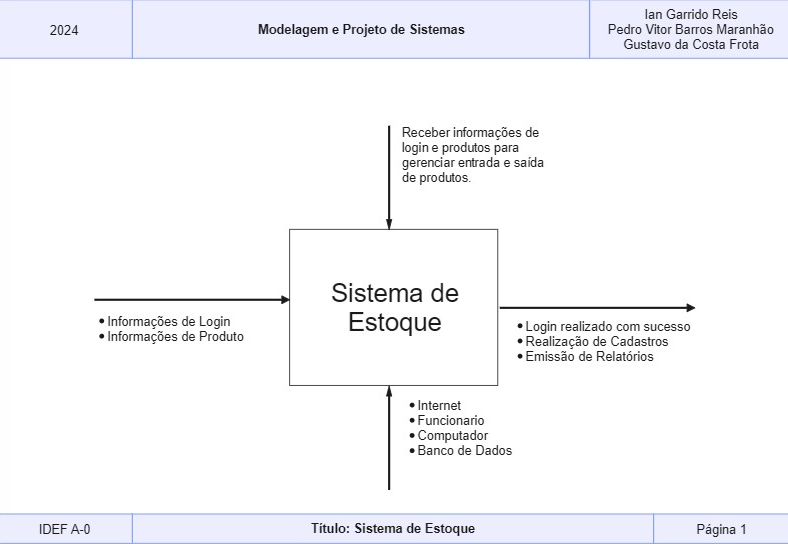
\includegraphics[width=0.8\linewidth]{figures/idefa-0.png}
        \label{fig:figura1}
    \end{figure}

    \begin{figure}
        \centering
        \caption{IDEF A01 referente ao projeto.}
        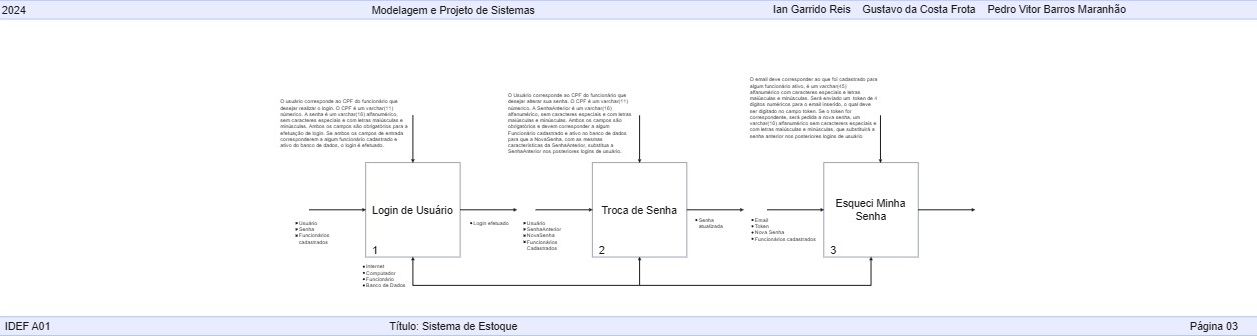
\includegraphics[width=0.8\linewidth]{figures/idefa01.png}
        \label{fig:figura2}
    \end{figure}
 
    \begin{figure}
        \centering
        \caption{Diagrama de Caso de Uso referente ao projeto.}
        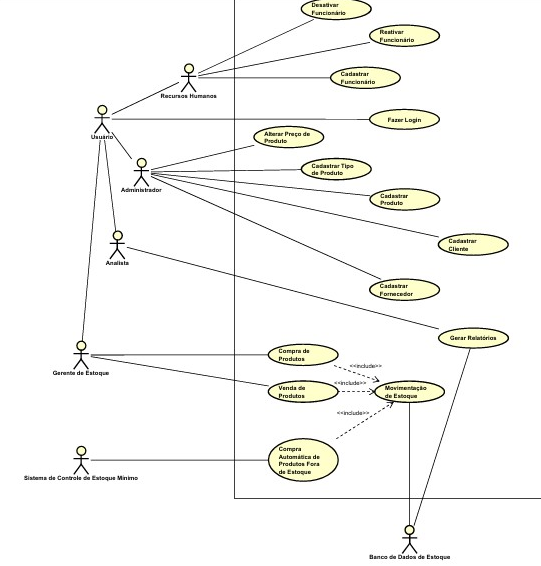
\includegraphics[width=0.8\linewidth]{figures/diagramaUC.png}
        \label{fig:figura3}
    \end{figure}
    
    \begin{figure}
        \centering
        \caption{Diagrama de Sequência para o caso de uso Compra de Produtos referente ao projeto.}
        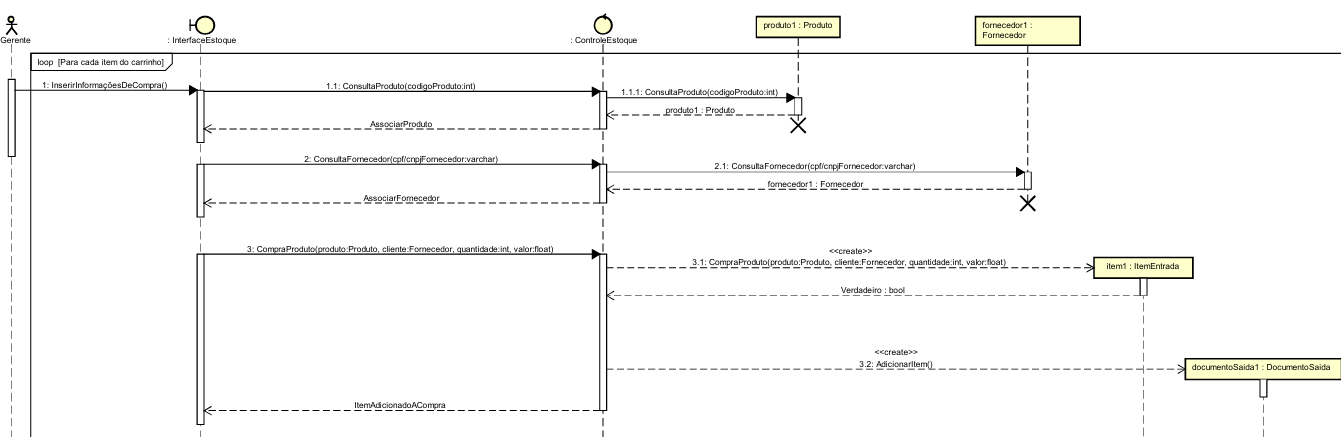
\includegraphics[width=0.8\linewidth]{figures/diagramaSequencia.png}
        \label{fig:figura4}
    \end{figure}
 
    \begin{figure}
        \centering
        \caption{Diagrama de Atividades para o caso de uso Compra de Produtos referente ao projeto.}
        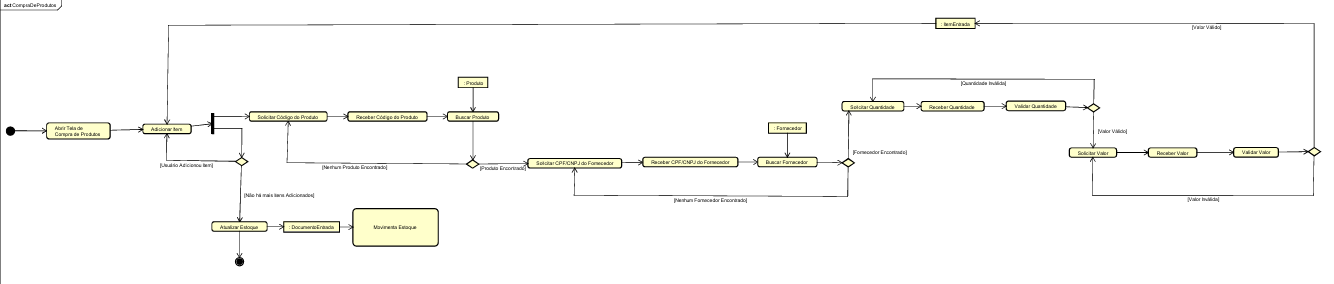
\includegraphics[width=0.8\linewidth]{figures/diagramaAtividades.png}
        \label{fig:figura5}
    \end{figure}
 
    \begin{figure}
        \centering
        \caption{Diagrama de Implantação referente ao projeto.}
        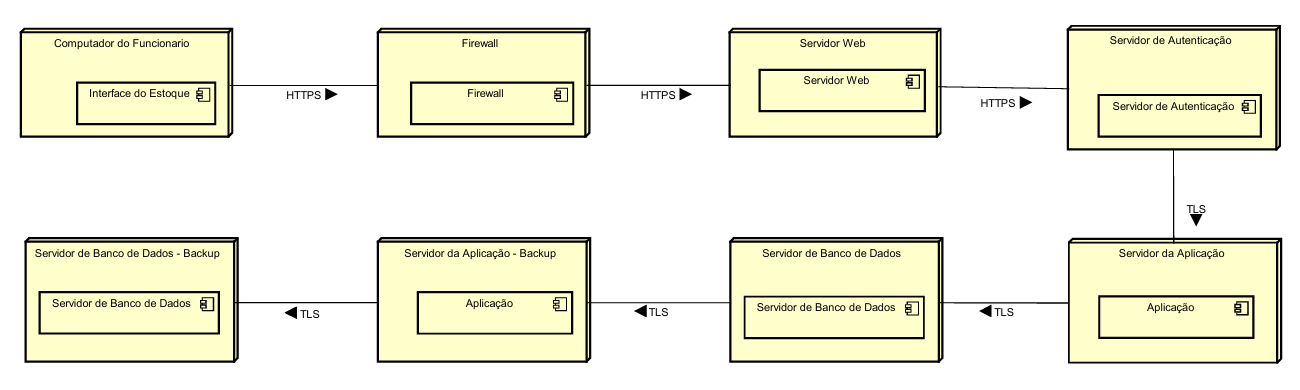
\includegraphics[width=0.8\linewidth]{figures/diagramaImplantacao.png}
        \label{fig:figura6}
    \end{figure}

    \begin{figure}
        \centering
        \caption{Diagrama de Classes referente ao projeto.}
        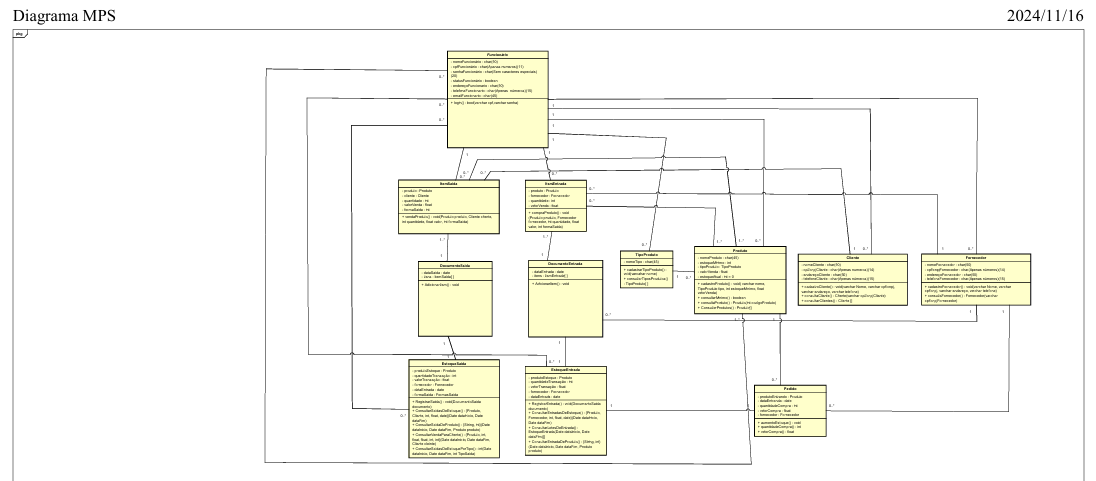
\includegraphics[width=0.8\linewidth]{figures/diagramaClasse.png}
        \label{fig:figura7}
    \end{figure}
 
    \begin{figure}
        \centering
        \caption{Modelagem de Banco de Dados Físico referente ao projeto.}
        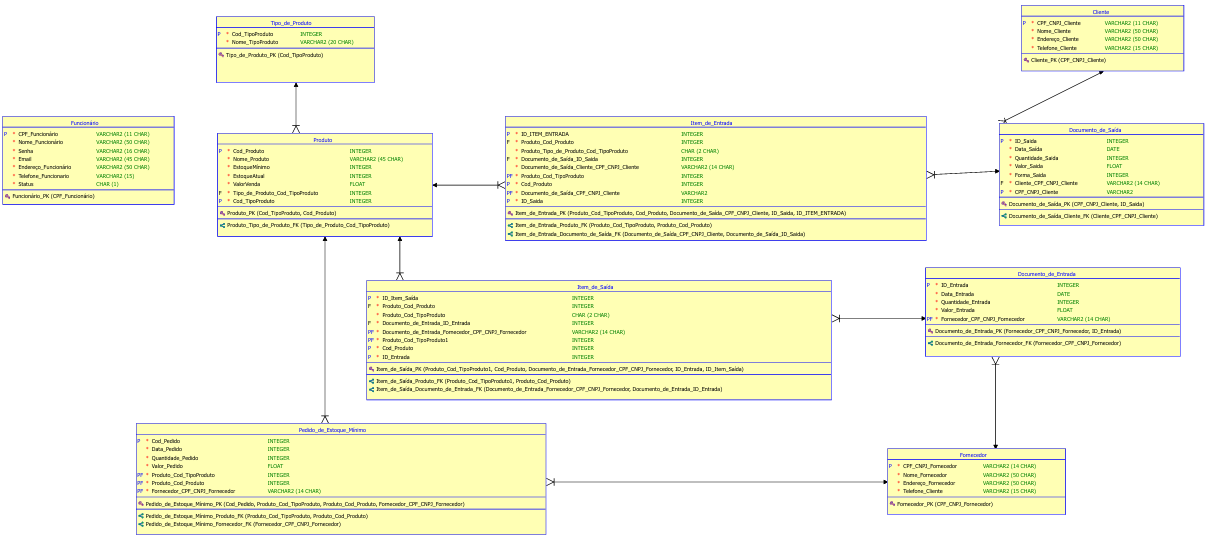
\includegraphics[width=0.8\linewidth]{figures/modeloBDFisico.png}
        \label{fig:figura8}
    \end{figure}
    
    \begin{figure}
        \centering
        \caption{Modelagem de Banco de Dados Lógico referente ao projeto.}
        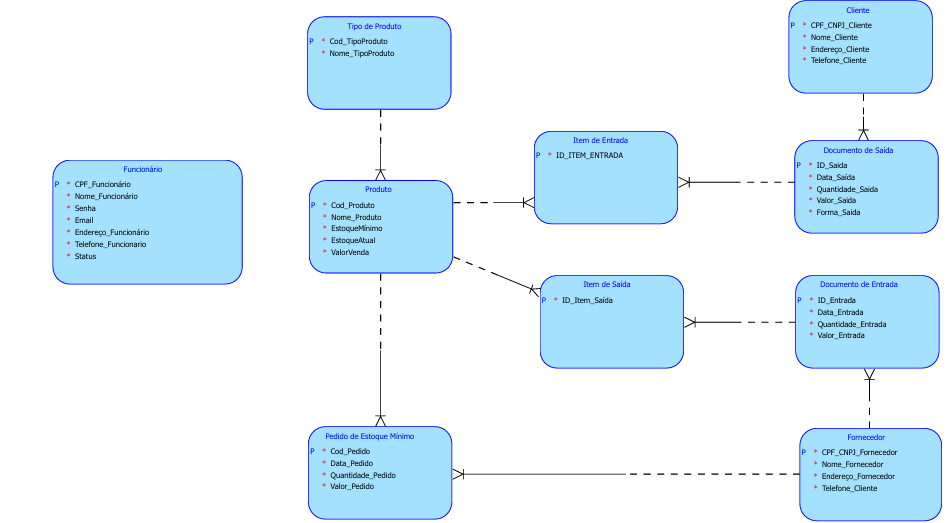
\includegraphics[width=0.8\linewidth]{figures/modeloBDLogico.png}
        \label{fig:figura9}
    \end{figure}

    \begin{figure}
        \centering
        \caption{Certificado de conclusão do projeto Academia STEM pelo pilar Permanência.}
        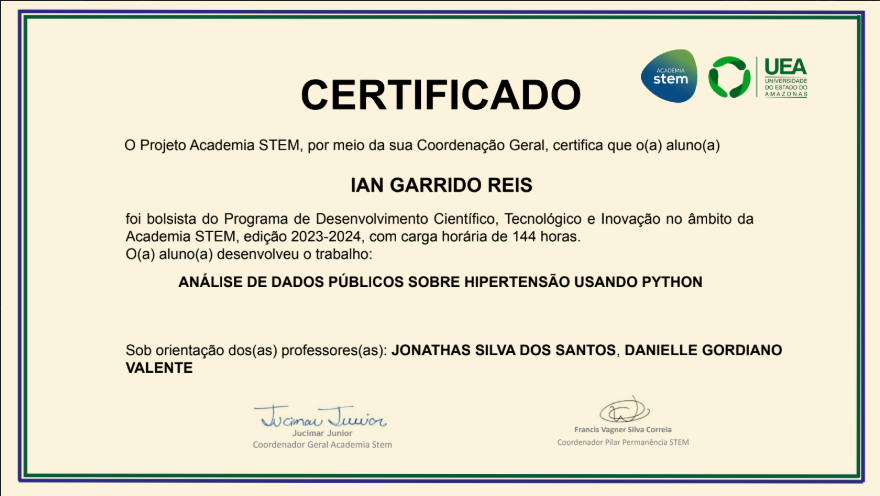
\includegraphics[width=0.8\linewidth]{figures/certificado.png}
        \label{fig:figura10}
    \end{figure}

\end{document}